\subsection{Design and verification of a L-shaped lug wrench}
	\paragraph{Problem} A lug wrench is the name for a type of socket wrench used to loosen and tighten lug nuts on automobile wheels; lug wrenches may be L-shaped (as in this case) or $X$ shaped. Design and verify such component considering the following product design specification:
	\begin{center}
		\rule{0.8\linewidth}{1.5pt} \\
		\textbf{Product Design Specifications} \\
		\label{tab:scf-firstiter}
		\begin{tabular}{ p{0.2cm} p{8cm} c c  }
			& Specification & Symbol & Value \\ \hline 
			\multicolumn{2}{l}{1) Geometry} \\
			& 1.1) working distance from vehicle & $a_{min}$ & $200mm$ \\
			& 1.2) maximum weight & $m_{max}$ & $1kg$ \\
			\multicolumn{2}{l}{2) Loads} \\
			& 2.1) preload torque & $T$ & $120 N\cdot m$ \\
			& 2.2) user nominal force & $F_{nom}$ & $300N$ \\
			& 2.3) user maximum force & $F_{max}$ & $1\,000N$ \\
			\multicolumn{2}{l}{3) Deflections} \\
			& 3.1) maximum deflection under nominal load & $\delta_{max}$ & $14mm$ \\
			\multicolumn{2}{l}{4) Material} \\
			& 4.1) corrosion resistant & & medium \\
			& 4.2) cost & & low \\
			& 4.3) yield strength & $\sys$ & high \\
		\end{tabular}
		\rule{0.8\linewidth}{1.5pt}
	\end{center}
	
	\paragraph{Solution} Considering the schematic representation of the lug wrench in figure \ref{ex:lug-a}, the first thing to do is determining the minimum value of the length $b$; this can be obtained considering that, in nominal condition, the torque generated by the applied force $F$ must equate the preload $T$ of the lug nuts, thus
	\[ T = F b \qquad \Rightarrow \qquad b_{min} = \frac{T}{F_{nom}} = 400mm \]
	
	\begin{SCfigure}[1.5][b]
		\centering 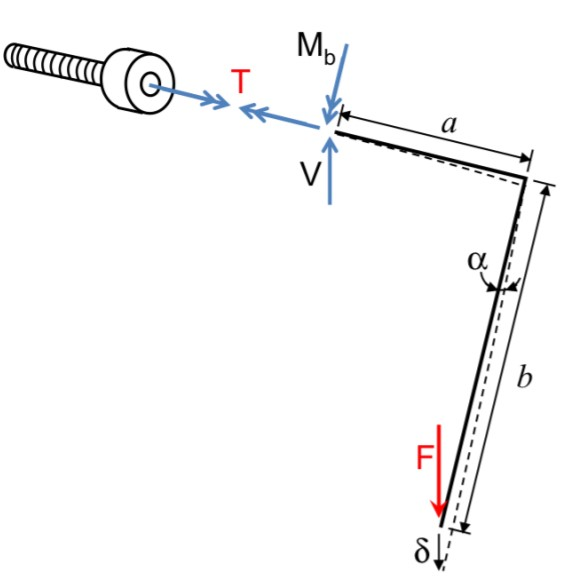
\includegraphics[width=5cm]{lug-a}
		\caption{free body diagram of the L-shaped lug wrench.} \label{ex:lug-a}
	\end{SCfigure}
	
	Considering from now on (in order to reduce the mass) the minimum dimension for the structure $a = a_{min} = 200mm$ and $b = b_{min} = 400mm$, the next step in order to proceed with the design is determining the internal actions.	
	\begin{figure}[bt]
		\centering
		\begin{subfigure}{0.48\linewidth}
			\centering 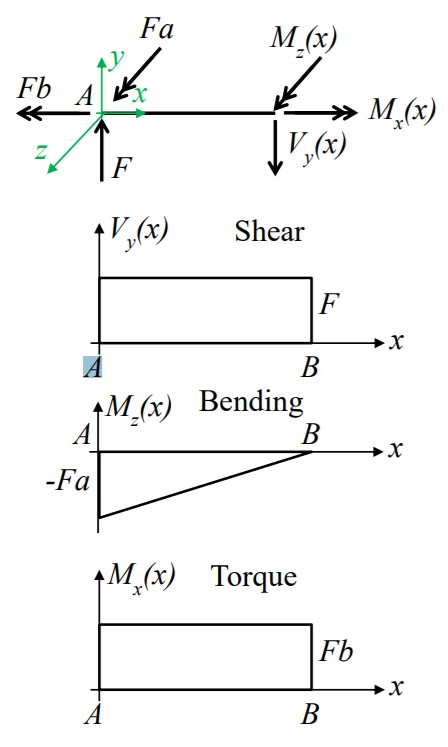
\includegraphics[width=4cm]{lug-b} \caption{}
		\end{subfigure}
		\begin{subfigure}{0.48\linewidth}
			\centering 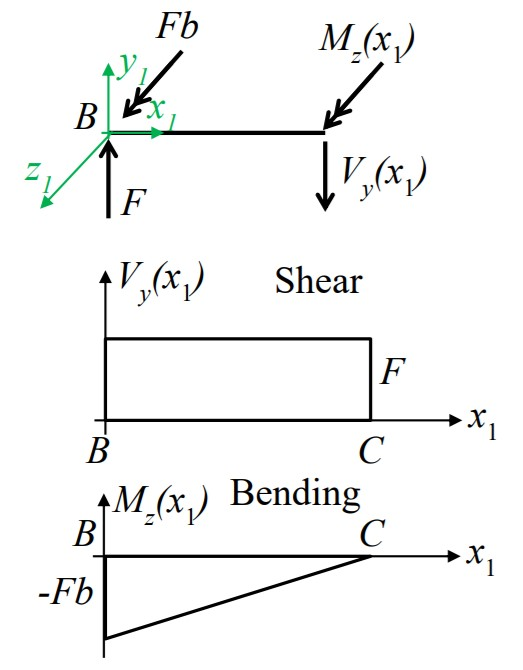
\includegraphics[width=4cm]{lug-c} \caption{}
		\end{subfigure}
		\caption{internal loading diagrams for the first section with length $a$ (fig a) and length $b$ (fig. b).} \label{ex:lug-b}
	\end{figure}
	The results as reported in figure \ref{ex:lug-b} present a constant shear of magnitude $F$ throughout the structure and so a \textit{triangular shaped} bending moment. The bid that's attached to the nut is also subjected to torsional load equal to $Fb$.
	
	The chosen material compatible with the product design specification can the \texttt{51CrV4}, a low-cost, high-strength and corrosion resistant steel used for springs and tools whose properties are
	\[ E = 205GPa \qquad \nu = 0.3 \qquad \sys = 800 MPa \qquad \suts = 1\,000 MPa \qquad \rho = 7\,850 kg/m^3  \]
	
	A strategy for dimensioning the first bead of the lug wrench (AB) subjected to torsion is by using a hollow circular section with internal diameter $d_i$ and external $d_e$. For such section
	\[ A = \frac\pi 4 \big(d_e^2-d_i^2\big) \hspace{2cm} I_x = I_y = \frac{\pi}{64} \big(d_e^4-d_i^4\big) \hspace{2cm} J_p = I_x + I_y = \frac \pi {32} \big(d_e^4-d_i^4\big) \] 
	and so the stress states due to bending $\sigma_{zz}$ and torsion $\tau_{\lambda z}$ can be computed as
	\[ \szz = \frac{M_x}{I_x} \frac{d_e}{2} \hspace{3cm} \tlz = \frac{M_z}{J_p} \frac {d_e}2 \]
	Using Von-Mises equivalent stress 
	\[ \seq = \sqrt{\szz^2 + 3\tlz^2} = \sqrt{\frac{1\,024 d_e^2}{\big(d_e^4-d_i^4\big)^2 \pi^2} (F_{max}a)^2 + \frac{768 d_e^2}{\big(d_e^4-d_i^4\big)^2\pi^2} (F_{max}b)^2 } \leq \frac{\sys}{\phi} \]
	Assuming a safety factor $\phi = 1.5$, after iterative solution it can be obtained the solution
	\[ d_i = 21mm \hspace{3cm} d_e = 25mm \]
	with moments of area $I_x = I_y = 9\,628,2mm^4$ and polar moment $J_p = 19\,256.4mm^4$.
	
	The second section $BC$ of the lug wrench is mainly subjected to bending load and a good design choice can be a hollow rectangular section; considering the walls to have equal thickness $s = 2mm$ (equal to the thickness of the hollow circle just found) and dimension \textit{measured from the outside} $B\times H$, then the moment of inertia $I_x$ that bear the bending is computed as
	\[ I_x = \frac{BH^3}{12} - \frac{(B-2s)(H-2s)^3}{12} \]
	Considering that at point $B$ we have only bending with a maximum value of $M_x = F_{max} b$, in order to properly dimension the section we have to chose $B,H$ such that
	\[ \szz = \frac{F_{max} b}{I_x} \frac H 2 \leq \frac \sys \phi \]
	and so a candidate that full-fills the requirement is $B = 10mm, H=28mm$ having moment of inertia $I_x = 11\,381.3mm^{4}$.
	
	With the stress verification passed it's possible to do a stiffness check to verify that the deflection of the lug wrench, in nominal load condition, doesn't exceed $\delta_{max}$. Such problem can be solved using Castigliano's theorem: the elastic internal energy of the system is
	\begin{align*}
		U_e & = \int_0^a \frac{M_x^2}{2 E I_{x,AB}} dz + \int_0^a \frac{M_z^2}{2GJ_t}\, dz + \int_a^b \frac{M_x^2}{2 E I_{x,BC}}\, dz \\
		& = \int_0^a \frac{F^2(a-z)^2}{2 E I_{x,AB}} dz + \int_0^a \frac{F^2b^2}{2GJ_t}\, dz + \int_0^b \frac{F^2(b-z)^2}{2 E I_{x,BC}}\, dz \\
		& = \frac{a^3F^2}{6 E I_{x,AB}} + \frac{a b^2 F^2}{2G J_p} + \frac{b^3F^2}{6 E I_{x,BC}}
	\end{align*}
	hence the deflection
	\[ \delta_F = \frac{\partial U_e}{\partial F} = \left( \frac{a^3}{3 E I_{x,AB}} + \frac{a b^2}{G J_p} + \frac{b^3}{3 E I_{x,BC}} \right) F  \]
	Having the shear modulus $G = \frac E{2(1+\nu)} = 78.8 GPa$, the displacement in the case of nominal force applied is $\delta_{F,nom} = 9.47mm$ that's lower then the admissible value of $14 mm$ stated in the product design specification. 
	
	Lastly we have to verify that the structure is compliant respect to weight (to lug shouldn't overcome the $1kg$ threshold); knowing the density $\rho$ of the material we have
	\[ m = \frac \pi 4 \big(d_e^2-d_i^2\big) a \rho + \Big(BH - (B-2s)(H-2s)\Big) b \rho = 0.65 kg < 1kg  \]
	
	
	
	
	
	
	
	
	
	
	
	
	
	
	
	
	
	
	
	
	
	
	